% Standalone TikZ figure — latexmk -pdf -outdir=build tikz-standalone.tex
% Include the resulting PDF from the main doc: 
\includegraphics{fig/tikz-standalone.pdf}
\documentclass[tikz, border=2pt]{standalone}
\usetikzlibrary{positioning, arrows.meta}

\begin{document}
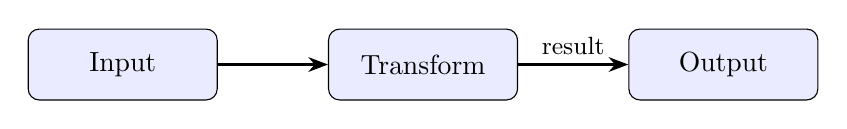
\begin{tikzpicture}[
  node distance = 8mm and 14mm,
  box/.style = {draw, rounded corners, minimum width=2.4cm, minimum height=9mm,
                align=center, fill=blue!8},
  arr/.style = {-{Stealth[length=2.5mm]}, thick},
]
  \node[box] (in)  {Input};
  \node[box, right=of in]  (mid) {Transform};
  \node[box, right=of mid] (out) {Output};

  \draw[arr] (in)  -- (mid);
  \draw[arr] (mid) -- (out) node[midway, above] {\small result};
\end{tikzpicture}
\end{document}
